\documentclass{article}  % univerzitná trieda 

% ===== Kódovanie a jazyk =====
\usepackage[utf8]{inputenc}
\usepackage[IL2]{fontenc}        % lepšie písmeno Ľ
\usepackage[slovak]{babel}

% ===== Grafika a PDF =====
\usepackage{graphicx}
\usepackage{url}                 % príkaz \url na formátovanie URL
\usepackage{pdfpages}            % vloženie PDF
\usepackage{hyperref}            % aktívne odkazy

% ===== Titulka =====
\title{Názov semestrálnej práce}
\author{Yaroslav Nesteruk \\ 
        {\small Slovenská technická univerzita v Bratislave} \\ 
        {\small Fakulta informatiky a informačných technológií} \\ 
        {\small \texttt{...@stuba.sk}}}
\date{07. október 2025}

\begin{document}
\maketitle

% ===== Úvod =====
\section{Úvod}
Umelá inteligencia (AI) sa stala jednou z najdynamickejšie sa rozvíjajúcich oblastí informatiky. 
Jej vplyv siaha od priemyslu až po každodenný život. Cieľom tejto práce je zhrnúť základné princípy, 
metódy a smerovanie moderného výskumu v tejto oblasti.

% ===== Ciele práce =====
\section{Ciele práce}
Cieľom práce je analyzovať aktuálne trendy v oblasti umelej inteligencie a poukázať na ich praktické 
uplatnenie v rôznych odvetviach – od medicíny po dopravu.

% ===== Použité metódy =====
\section{Použité metódy}
Pri spracovaní práce boli použité metódy:
\begin{itemize}
    \item Analýza odborných publikácií
    \item Porovnanie výsledkov experimentov
    \item Syntéza poznatkov z viacerých zdrojov
\end{itemize}

% ===== Výsledky a diskusia =====
\section{Výsledky a diskusia}
Na základe štúdia relevantných zdrojov možno pozorovať, že najrýchlejší rozvoj nastáva v oblastiach 
neurónových sietí a generatívnych modelov. Veľkú pozornosť si zaslúži aj oblasť etiky AI – otázky súkromia, 
zaujatosti a transparentnosti algoritmov.

% ===== Príloha PDF =====
\section{Príloha PDF}
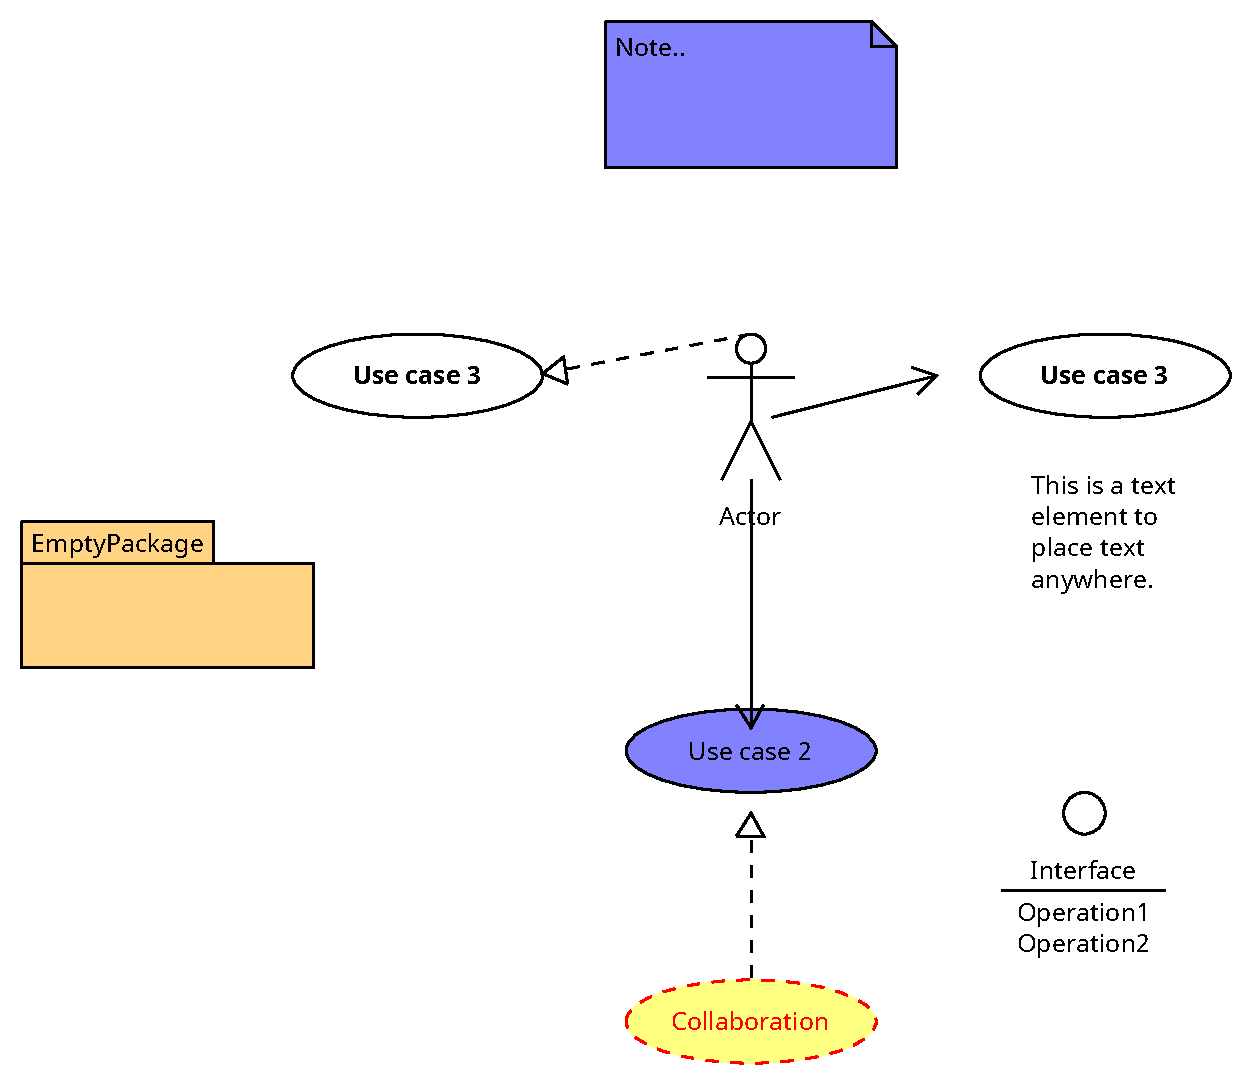
\includepdf[pages=-]{diagram_AI_architektura.pdf}
 % vloží všetky strany PDF

% ===== Záver =====
\section{Záver}
Umelá inteligencia bude v nasledujúcich rokoch zohrávať kľúčovú úlohu vo všetkých sférach spoločnosti. 
Preto je potrebné venovať pozornosť nielen technickému rozvoju, ale aj spoločenským dopadom tejto technológie.

% ===== Literatúra =====
\section{Literatúra}
\begin{thebibliography}{9}
\bibitem{Goodfellow2016}
Ian Goodfellow, Yoshua Bengio, Aaron Courville. \emph{Deep Learning}. MIT Press, 2016.

\bibitem{Russell2010}
Stuart Russell, Peter Norvig. \emph{Artificial Intelligence: A Modern Approach}. Pearson, 2010.

\bibitem{EthicsAI2021}
Floridi, L. a kol. \emph{Ethics of Artificial Intelligence: Principles and Practice}. Oxford University Press, 2021.
\end{thebibliography}

\end{document}
